% 2020 江苏卷 15：三棱柱 ABC-A1B1C1，E、F 分别为 AC、B1C 的中点
% 绘制依据：固定源 PDF 第 1115 面原图。斜置三棱柱：底面三角形 A 左、B 前下、C 右，
% A1、B1、C1 分别位于 A、B、C 的正上偏右（同一平移向量）。可见棱实线，隐蔽棱虚线。
% 图中另画出 AB1（实线）与 AC1（虚线，体内对角线），E 在 AC 上、F 在 B1C 上。
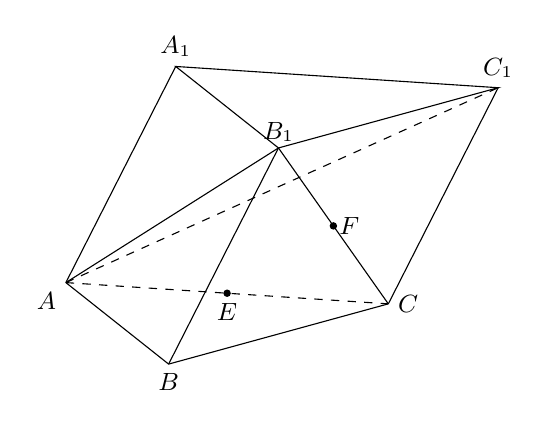
\begin{tikzpicture}[scale=0.9, font=\small]
  \coordinate (A) at (0,0);
  \coordinate (B) at (1.45,-1.15);
  \coordinate (C) at (4.55,-0.30);
  \coordinate (A1) at (1.55,3.05);
  \coordinate (B1) at (3.00,1.90);
  \coordinate (C1) at (6.10,2.75);
  \coordinate (E) at (2.275,-0.15);
  \coordinate (F) at (3.775,0.80);

  % 底面三角形
  \draw (A) -- (B) -- (C);
  \draw[dashed] (A) -- (C);
  % 侧棱
  \draw (A) -- (A1);
  \draw (B) -- (B1);
  \draw (C) -- (C1);
  % 顶面三角形
  \draw (A1) -- (B1) -- (C1) -- cycle;
  % 题设涉及的线段：AB1 实线，AC1 体内对角线（虚线），B1C 实线
  \draw (A) -- (B1);
  \draw[dashed] (A) -- (C1);
  \draw (B1) -- (C);

  \fill (E) circle (1.5pt);
  \fill (F) circle (1.5pt);
  \node[below left] at (A) {$A$};
  \node[below] at (B) {$B$};
  \node[right] at (C) {$C$};
  \node[above] at (A1) {$A_1$};
  \node[above, inner sep=2pt] at (B1) {$B_1$};
  \node[above] at (C1) {$C_1$};
  \node[below=2pt, inner sep=1.5pt] at (E) {$E$};
  \node[right, inner sep=2pt] at (F) {$F$};
\end{tikzpicture}
